\chapter{Optimal Calibrations} \label{sec:OpCa_HLT}
\section{General} % FIXME: the sections structure should be re-arranged/intergrated into the main general structure (the Introduction.tex part was untouched)

%% General
% From NGT Proposal: 
The general goal of this task is to optimise the calibration procedures for the online HLT data-taking of the CMS detector. Task 3.4 involves leveraging advanced computing techniques, including AI-driven predictive models, while enhancing traditional CMS calibration methods. \\
Such an improvement is essential to push real-time analysis based on $\mathrm{R}^3$ software (Task 3.1) to the same accuracy that we typically achieve offline. One could then store high-quality high-level information, which implies a big save in terms of storage.\\
\newline
A conceptual design of the ultimate setup foreseen in the context of the $\mathrm{R}^3$  project is shown in  Fig.~\ref{fig:NGT-HLT_CalibrationWorkflow}. \\
The input rate of \SI{40}{\mega\hertz} LHC collisions will be processed by the hardware Level 1 trigger system (L1T), whose output is foreseen to be \SI{500}{\kilo\hertz} during Run-\num{4} and \SI{750}{\kilo\hertz} during Run-\num{5} data taking. \\
\newline
In order to ensure an \emph{Offline-like} quality of the reconstruction to enable some "quick and dirty" analyses using the reconstructed objects by the HLT, without requiring additional steps, a dedicated real-time calibration system will need to process the entirety of the L1T accept stream.\\  
A buffer composed of SSDs will temporarily store events from the data acquisition system after L1T event filtering, with a retention period of approximately 8 to 12 hours. This buffer ensures that events remain available until optimal calibrations can be derived for the entire dataset (for an actual discussion of the architectural layout of this system refer to Section \ref{sec:DAQIntegration}.)\\
\newline
Immediately after data-taking, a small fraction (a few percent) of the buffered data, selected via light filtering of the L1T bits, will be processed by an accelerated calibration workflow. This workflow focuses on deriving the most critical conditions required for the online event selection at the HLT.\\
Once these conditions are stored and all necessary calibrations are completed, the HLT processing of the buffered data will commence, ensuring optimal calibration and event reconstruction. \\
The $\mathrm{R}^3$ project foresees the HLT farm output rate in Run-\num{5} to be around \SI{10}{\kilo\hertz} of standard RAW data. RAW data refers to the minimally processed, detector-level information recorded during collisions, including raw hits, energies, and other measurements from the various detector subsystems. This data serves as the starting point for all higher-level offline reconstruction and analysis steps, allowing in principle multiple reconstruction passes with updated reconstruction software and calibrations.\\ Meanwhile, the entire set of events passing the Level-1 Trigger (L1T) Accept will be saved in \texttt{NanoAOD} format. \texttt{NanoAOD} is a highly compact, flat ntuple format designed to store reconstructed physics objects (such as tracks, leptons, and jets) and their properties, as determined by the High-Level Trigger (HLT). This format enables efficient storage and rapid analysis by including only the essential physics information for downstream studies.

% Deliverable/milestone: Production of a report illustrating the current calibration workflows in CMS and evaluating the impact of non-optimal calibrations on the physics performance of the online reconstruction.

\begin{figure}[h!]	
\centering
\includegraphics[width=\textwidth]{figures/NGT-HLT_Calibration_Workflow.pdf} %\hfill
\caption{Conceptual Design of $\mathrm{R}^{3}$ Optimal Calibrations (NGT-HLT Calibration Workflow)}
\label{fig:NGT-HLT_CalibrationWorkflow}
\end{figure}

\section{Calibration Workflows Analysis}
In this section we conduct a comprehensive analysis of the current calibration workflows and procedures within CMS currently in place, highlighting the intricacies of the process, and identifying areas for improvement (bottlenecks) in the calibration process. 
The current preliminary survey focused on finding viable candidates for the prototype. A continued and more detailed follow-up survey is being planned, especially in the context of Phase 2 calibrations, including new detectors (MTD, HGCAL, new tracker, etc.)

%\include{chapters/Calibrations_General}
\subsection{Beamspot Calibration}

\subsubsection{Beamspot overview}

The \emph{beamspot} in CMS is the luminous region where the two beams interact.
This region is described by a probability density function $\rho(x,y,z)$ for the pp collisions;
to first approximation, the $\rho$ is given by a three-dimensional gaussian function that can be visualised as a tri-axial ellipsoid \cite{CMS-PAS-TRK-10-005}.
In ideal conditions, the beamspot would be centered in,
and its axes would be aligned to,
to the detector's reference frame.
During real operation, the beamspot is displaced and rotated along all axes,
which are represented by a displacement vector and a set of Euler angles.
Those quantities can be translated to the following observables, the \emph{beamspot parameters}:
\begin{itemize}
\item the centroid position $x_{\text{BS}}, y_{\text{BS}}, z_{\text{BS}}$,
\item the transverse widths $\sigma_{x}, \sigma_{y}$,
\item the longitudinal width $\sigma_{z}$,
\item and the tilts with respect to the $z$ axes: $\frac{dx}{dz}$, $\frac{dy}{dz}$.
\end{itemize}
Figure~\ref{fig:beamspotCartoon} shows the a diagram of the ideal and real beamspot.
\begin{figure}[htbp]
   \centering
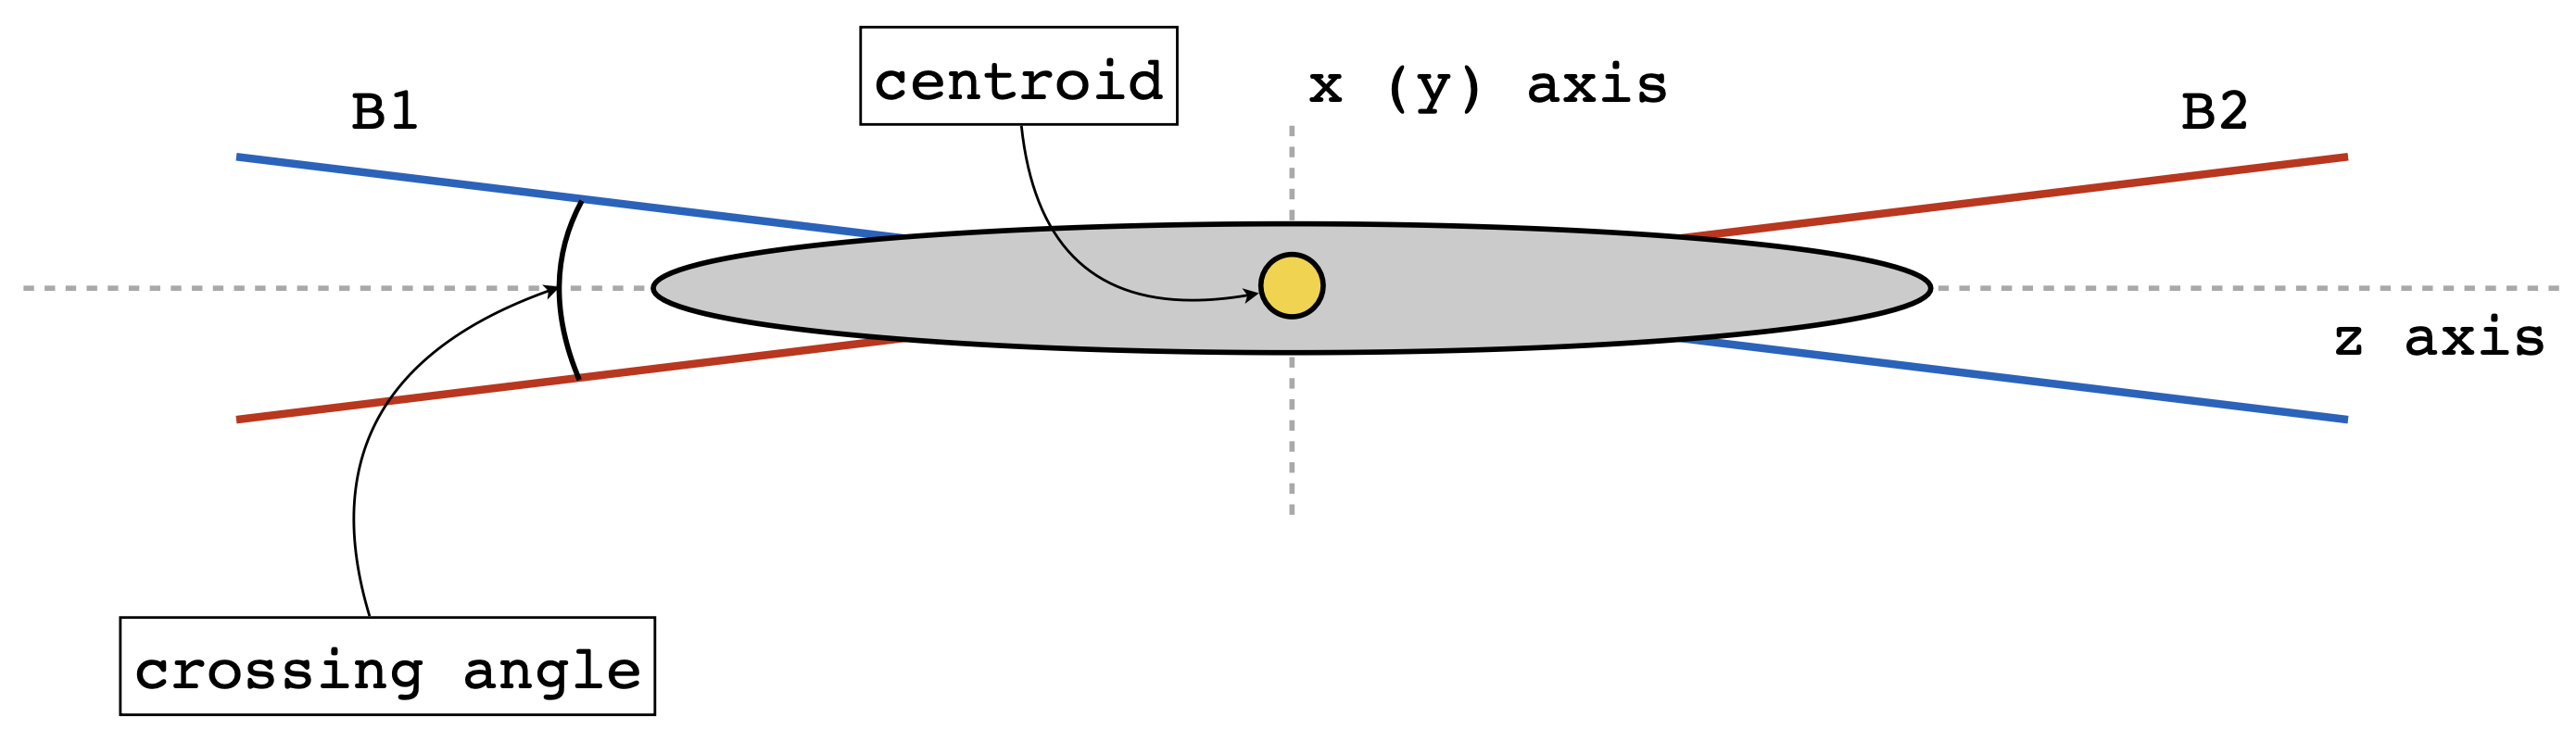
\includegraphics[width=0.7\textwidth]{figures/IdealBeamspot.png}\\[2ex]
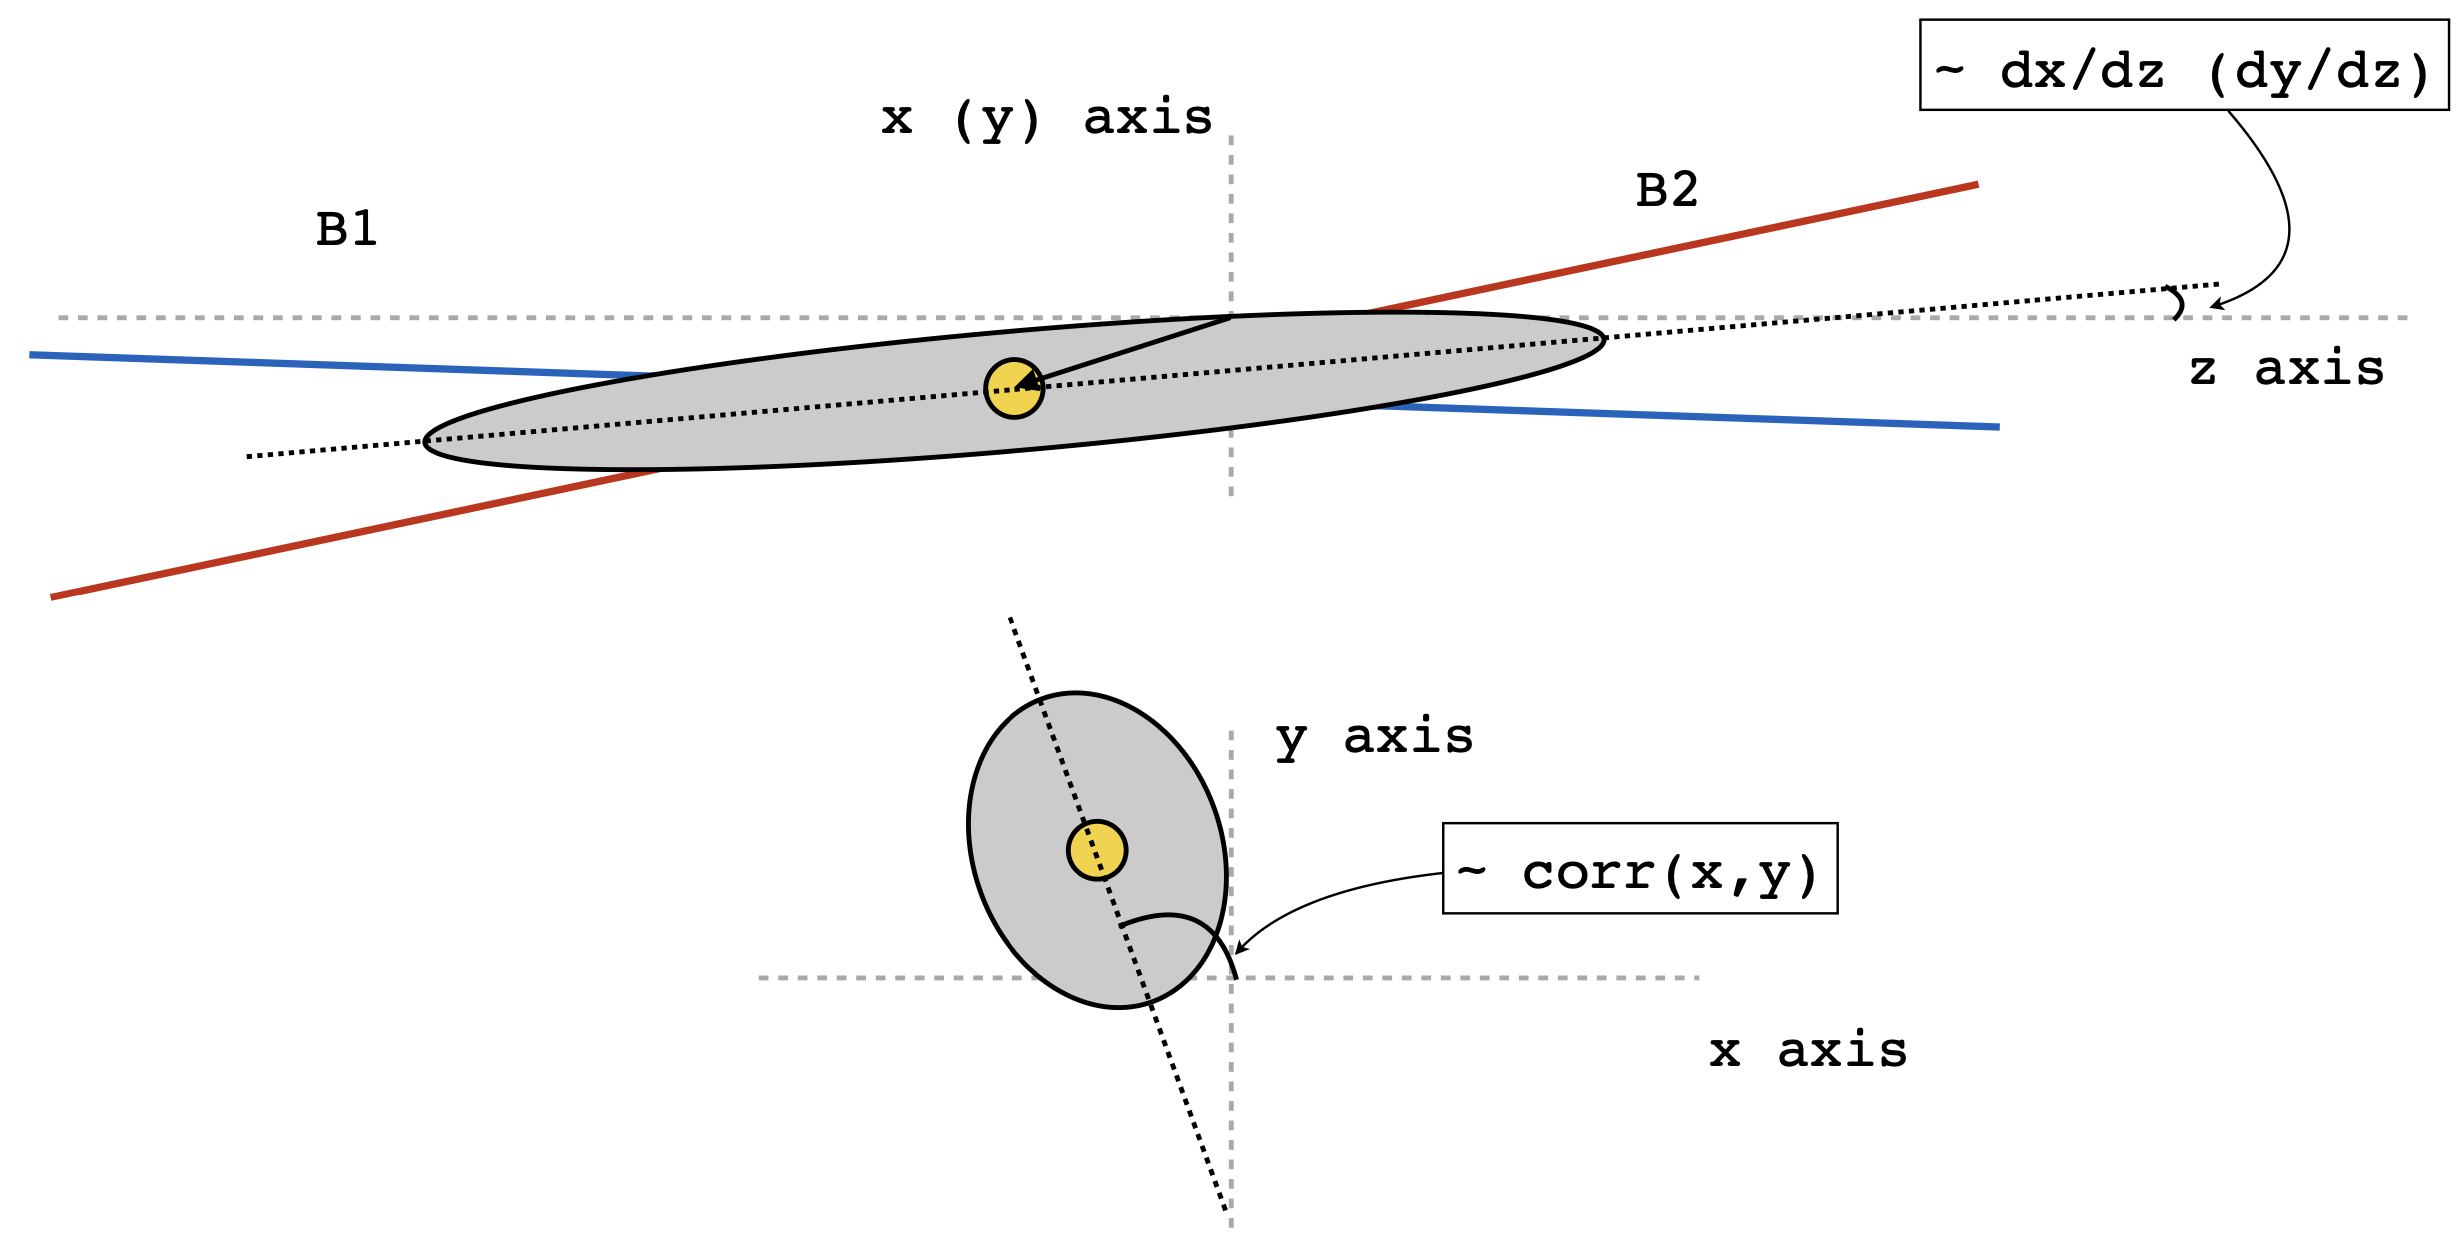
\includegraphics[width=0.7\textwidth]{figures/RealBeamspot.png}
   \caption{Diagram of the ideal (top) and real (bottom) beamspot.}
   \label{fig:beamspotCartoon}
\end{figure}

We determine the beamspot parameters by fitting track and vertex quantities for every lumi section.
The centroid position in the transverse plane and the tilts are obtained from a fit to the reconstructed tracks;
this is a $\chi^2$ fit that employs the track $d_0$--$\phi$ correlation:
\[
d_0(\phi_0, z_p) = x_{\text{BS}} \cdot \sin \phi_0 + \frac{dx}{dz} \cdot \sin\phi_0 \cdot z_p - y_{\text{BS}} \cdot \cos \phi_0 - \frac{dy}{dz} \cdot \cos \phi_0 \cdot z_p.
\]
as seen in Fig.~\ref{fig:trackD0Correlation}.

\begin{figure}[htbp]
   \centering
   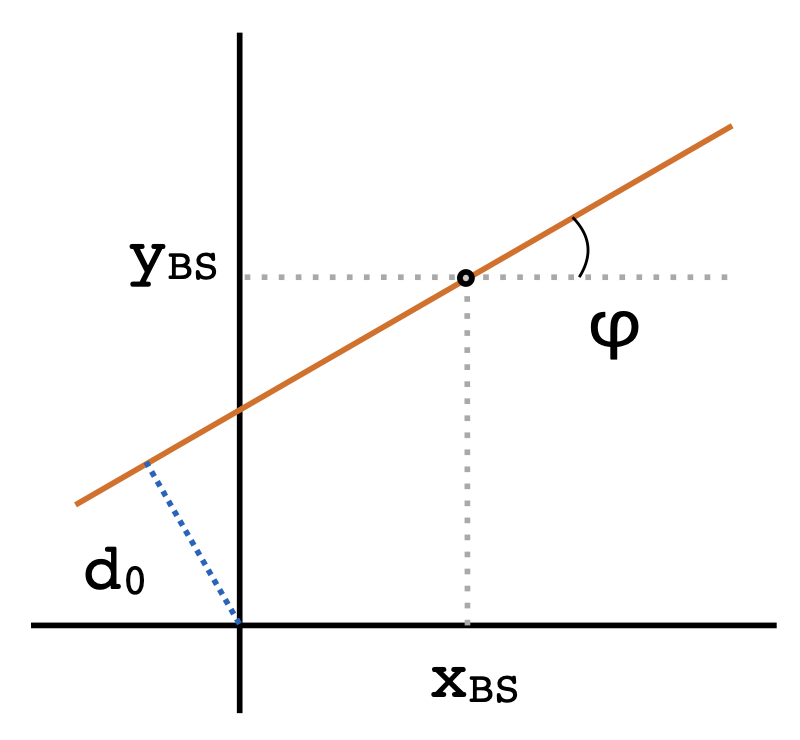
\includegraphics[width=0.5\textwidth]{figures/trackD0PhiCorrelation.png}
   \caption{The track $d_0$--$\phi$ can be used to measure the centroid position in the transverse plane and the centroid tilts.}
   \label{fig:trackD0Correlation}
\end{figure}

On the other hand,
the position along the $z$ axis and the beam widths are measured from a fit to the reconstructed vertices;
this is a maximum likelihood fit of a three-dimensional gaussian to the reconstructed vertices:
\[
\mathcal{L}=\sum_{\text {vertices }}-\ln \left(\frac{1}{\sqrt{(2 \pi)^3\left|\Sigma_{\text {tot }}\right|}} \cdot e^{-\frac{1}{2}(x-\mu)^T \Sigma_{\text {tot }}^{-1}(x-\mu)}\right)
\]
where $\Sigma_{\text {tot }} = \Sigma_{\text {beam }}^{\text {CMS }} + \Sigma_{\text {vtx }}$, with
$\Sigma_{\text {beam }}^{\text {CMS }}$ the beamspot widths in CMS's frame and
$\Sigma_{\text {vtx }}$ the vertex covariance matrix, different for every vertex.
Notice that $\Sigma_{\text {beam }}^{\text {CMS }}$ is rotated with respect to the beamspot principal axes:
\[
\Sigma_{\text {beam }}^{\text {CMS }}=R^T(\alpha, \beta, \gamma) \cdot \Sigma_{\text {beam }} \cdot R(\alpha, \beta, \gamma)
\]
where the $\alpha$ ($\beta$) rotation is along the $x$ ($y$) axis, and can be measured from $\frac{dy}{dz}$ ($\frac{dx}{dz}$).
The $\gamma$ rotation is negligible because the $xy$ correlation of the beams is very small.
The beamspot widths $\sigma_x$, $\sigma_y$, $\sigma_z$ are then given by the square roots of the diagonal elements of $\Sigma_{\text {beam }}$.

\subsubsection{Beamspot workflows}

There are separated workflows for
online usage (in the HLT) and
offline usage (in the prompt reconstruction).
In the online case, there are again two separated workflows, both running in the DQM farm:
the \emph{HLT client} fit uses the the full tracks and vertices reconstructed in the HLT, whilst
the \emph{legacy client} fit uses pixel-only tracks and vertices fitted in the DQM clients themselves.
In both cases the payload is obtained through moving average over a five lumisections sliding window.
These payloads are uploaded to CondDB in a DQM "O2O-like" workflow,
and
are consumed both by the HLT processing and by the Express reconstruction.
In the HLT the conditions are fetched every five lumisections.
This workflow has an arbitration mechanism (via an \texttt{ESProducer}) between old and new payloads for dynamic selection, and the system is triggered whenever a tag is updated, ensuring robust operations.
The system also contains fallback mechanisms for edge cases:
\begin{itemize}
\item unavailability of tracks from the HLT,
\item failure of the beam fit,
\item long times since the last payload upload (default threshold: 1 day),
\item LHC machine transitions (\textit{e.g}., LS, TS, MD, pp $\leftrightarrow$ HI),
\item possibility of ``dummy'' beamspot / beamspot with inflated uncertainties if necessary.
\end{itemize}
In the offline case there are four PCL workflows.
The \emph{high purity} workflow runs off a set of well-measured vertices from a stream of high \HT events,
with stringent requirements on vertex \PT and number of tracks, whils
the \emph{legacy} workflow runs on the regular Express stream and has minimal requirements on its inputs.
Both workflows have tags with lumisections and run granularity;
the standard tag used for prompt reconstruction is the high-purity by-lumisection tag, \texttt{BeamSpotObjects\_PCL\_byLumi\_v0\_prompt}.

\subsubsection{Recommendations}

In view of the above discussion, the beamspot would be a natural candidate for the NGT calbirations.
Ideally we would like to bring the high-purity by-lumisection workflow to the online system,
but it is known that the pressure on the conditions delivery system may be problematic (hence the five-lumisection granularity).

%The Beamspot online workflow has been updated in Run 3 to address the absence of the SCAL system.\\
%This does not affect the actual fit to tracks or primary vertex distributions but modifies the infrastructure for handling BeamSpot information. Key changes include:
%\begin{itemize}
%    \item Replacement of SCAL-based processes.
%    \item Improved workflow and fallback mechanisms for edge cases.
%    \item Arbitration between old and new payloads for dynamic selection.
%\end{itemize}

%The old Run 2 workflow consisted in the following steps:
%\begin{itemize}
%    \item BeamSpot clients dumped data to text files processed through the SCAL system.
%    \item Data was forwarded to the DIP and HLT systems.
%\end{itemize}

%While the new workflow consists of the these steps:
%\begin{itemize}
%    \item SCAL system replaced by direct DB uploads.
%    \item An \texttt{ESProducer} arbitrates between BeamSpot payloads dynamically.
%    \item A fallback mechanism uses dummy values if no good payloads are available.
%    \item The system is triggered whenever a tag is updated, ensuring robust operations.
%\end{itemize}

%Failures in past workflows (e.g., due to unavailable tracks at HLT) necessitated a fallback mechanism. The %key features include:
%\begin{itemize}
%    \item Arbitration logic to decide between stored and new BeamSpot values.
%    \item Checks for fit convergence and recency of results.
%    \item Use of a 5-lumi-section sliding window for BeamSpot fits.
%    \item Ongoing studies on transverse widths, $\sigma_Z$, track counts, and PVs.
%\end{itemize}


%The new O2O mechanism ensures timely updates:
%\begin{itemize}
%    \item Automatically checks the time since the last payload upload (default threshold: 1 day).
%    \item Handles machine transitions (e.g., LS, TS, MD, pp $\leftrightarrow$ HI).
%    \item Uploads a "fake" BeamSpot object with inflated uncertainties if necessary.
%    \item Arbitration based on the time-of-creation of payloads, stored in \texttt{BeamSpotOnlineObjects}.
%\end{itemize}

%The updated Beam Spot online workflow addresses Run 3 requirements:
%\begin{itemize}
%    \item SCAL system replaced with DB uploads and fallback logic.
%    \item Successful implementation of O2O mechanisms for special machine transitions.
%    \item Ongoing work includes monitoring, fallback logic finalization, and integration with DIP.
%\end{itemize}
 % Marco / Thiago
\subsection{Pixel Tracker Calibrations}

The CMS Silicon Pixel detector is integral to the High-Level Trigger (HLT) decision-making process, as it provides information for the seeding of the charged particle tracking algorithm, as well as crucial information for the determination of the primary and secondary interaction vertices \cite{Dominguez:1481838,Adam_2021}.\\
This part of the report delves into the calibration prospects of the SiPixel detector, emphasising unused records, Front End Drive (FED) cabling, gain and quality calibrations, Cluster Position Estimator (CPE) conditions, and alignment practices.\\
Future prospects and recommendations for improving calibration workflows under the NGT framework are also discussed.\newline \newline 
Out of the 326 conditions in the HLT GT, 13 are related to the Silicon Pixel Tracker, of which 12 are relevant to Run 3 data-taking. From these, the following 8 are considered core and critical for data-taking:

\begin{table}[h!]
    \centering
    \begin{adjustbox}{max width=\textwidth}
    \begin{tabular}{p{2.5cm}|p{5.7cm}|p{1.5cm}|p{2.5cm}|p{3.0cm}}
        \textbf{Name} & \textbf{Record} & \textbf{Workflow} & \textbf{Frequency of Updates} & \textbf{Description} \\ \hline
      Lorentz Angle   & \texttt{SiPixelLorentzAngleRcd}                 & Manual & Typically a few times per year (mandatory when pixel HV changes) & Hall mobility per unit magnetic field strength\\ \hline
      Generic Errors  & \texttt{SiPixelGenErrorDBObjectRcd}             & Manual & Typically a few times per year (mandatory when pixel HV changes) & Uncertainty on the hit position \\ \hline
      1D-templates     & \texttt{SiPixelTemplateDBObjectRcd}             & Manual & Typically a few times per year (mandatory when pixel HV changes) & Cluster shape for hit position determination (1D)\\ \hline
      2D-templates    & \parbox[t]{5cm}{\texttt{SiPixel2DTemplateDBObjectRcd,}\\\texttt{numerator}} & Manual & Typically a few times per year (mandatory when pixel HV changes) & Cluster shape for hit position determination (2D)\\ \hline
      Bad channels    & \texttt{SiPixelQualityFromDbRcd}                & Manual & Typically a few times per year & Inventory of detector and readout defects \\ \hline
      Per-pixel Gains & \texttt{SiPixelGainCalibrationForHLTRcd}        & Manual & Once or twice per year & ADC to electron conversion factors \\ \hline
      Lorentz Angle   & \texttt{SiPixelLorentzAngleRcd,forWidth}        & Manual & Rarely (last update done in 2019) & Hall mobility per unit magnetic field strength \\ \hline
      Cabling map     & \texttt{SiPixelFedCablingMapRcd}                & Manual & Fixed for a given detector geometry & Readout to detector ID map \\ \hline
      Dead channels   & \texttt{SiPixelDetVOffRcd}                      & Manual & Not used & Inventory of unpowered channels \\ \hline
      Per-column Gains& \texttt{SiPixelGainCalibrationOfflineRcd}       & Manual & Not used & ADC to electron conversion factor \\ \hline
      Lorentz Angle   & \parbox[t]{5cm}{\texttt{SiPixelLorentzAngleRcd,}\\\texttt{fromAlignment}} & Manual & Not used & Hall mobility per unit magnetic field \\ \hline
      Bad channles    & \parbox[t]{5cm}{\texttt{SiPixelQualityFromDbRcd,}\\\texttt{forRawToDigi}} & Manual & Not used & Detector level defects \\ \hline
        
    \end{tabular}
    \end{adjustbox}
    \caption{Fundamental Silicon Strip Tracker Calibrations, ordered in terms of frequency of updates.}
    \label{tab:PixelCalibrations_critical}
\end{table}

\subsubsection{Unused Records in SiPixel Calibration}
Several records remain unused at HLT but hold relevance for other operational aspects:
\begin{itemize}
    \item \texttt{SiPixelDetVOffRcd}: Lists detector IDs with HV or LV off. Payload is ideal or empty.
    \item \texttt{SiPixelGainCalibrationOfflineRcd}: Stores gain and pedestal values for offline analysis.
    \item \texttt{SiPixelLorentzAngleRcd ("from alignment")}: Contains Lorentz Angle offsets, outdated since 2017.
    \item \texttt{SiPixelTemplateDBObjectRcd ("0T")}: Used during 0T templated tracking for PixelRecHits.
\end{itemize}

\subsubsection{FED Cabling and Calibration Maps}
The \texttt{SiPixelFedCablingMapRcd} records cabling maps connecting FEDs to readout channels. While not a direct calibration, this record plays a vital role in detector topology and reconstruction. This was last updated in 2017 with the transition to the Pixel Phase-1 detector.

\subsubsection{Bad components}
Description: This payload contains the module identification numbers (\texttt{DetId}) and readout chips (ROC)s numbers associated with those \texttt{DetID}s that are considered "dead." It is used by the track reconstruction algorithm.\\
Record Name: \texttt{SiPixelQualityRcd} 

\subsubsection{Pixel hit position reconstruction}

The position of a pixel cluster in the transverse (\(u\)) and longitudinal (\(v\)) directions on the sensor is determined by projecting the cluster onto the respective axis and summing the charge collected in pixels with the same coordinate \cite{Tracking_2014}. For single-pixel clusters, the position is the center of the pixel, corrected for Lorentz drift. For larger clusters, the hit position (\(u_{\text{hit}}\)) is computed using the relative charge in the first and last pixels of the projected cluster:

\begin{equation}
u_{\text{hit}} = u_{\text{geom}} + \frac{Q_{\text{last}} - Q_{\text{first}}}{2(Q_{\text{last}} + Q_{\text{first}})} |W_u - W_u^{\text{inner}}| - \frac{L_u}{2},
\end{equation}

where:
\begin{itemize}
    \item \(Q_{\text{first}}\), \(Q_{\text{last}}\): Charges in the first and last pixels of the cluster.
    \item \(u_{\text{geom}}\): Geometric center of the projected cluster.
    \item \(L_u/2 = D \tan \Theta_u^{\text{L}}/2\): Lorentz shift, with \(\Theta_u^{\text{L}}\) as the Lorentz angle and \(D\) as the sensor thickness.
    \item \(W_u^{\text{inner}}\): Geometrical width excluding the first and last pixels, zero for clusters smaller than three pixels.
    \item \(W_u = D \left| \tan (\alpha_u - \pi/2) + \tan \Theta_u^{\text{L}} \right|\): Charge width, derived from the track impact angle (\(\alpha_u\)) and Lorentz angle.
\end{itemize}

If no track is available, \(\alpha_u\) is assumed based on the particle's origin at the CMS detector center. The formula accounts for the partial charge deposition in the first and last pixels, estimating the extension of charge into these pixels (\(W_u - W_u^{\text{inner}}\)), which ranges between zero and twice the pixel pitch. This extension, combined with the relative charge, provides the edges of the charge distribution. The mean value of these edges, corrected for Lorentz drift, yields the cluster position.

For pixel barrel detectors, the Lorentz shift is approximately 59~\(\mu\)m.

\subsubsection{Pixel Lorentz Angle}
Description: The 'no label' payload contains the value of Lorentz Angle / Tesla for the Barrel Pixel and Forward Pixel separately (due to different high voltage (HV) constants, geometry, etc.).\\
Record Name: \texttt{SiPixelLorentzAngleRcd} 
Labels = none, \texttt{fromAlignment} or \texttt{forWidth} - given when included in a global tag.
\begin{itemize}
\item \texttt{fromAlignment} : the LA offset generated by alignment (alternative to LA correction from templates).
\item \texttt{forWidth}: the LA for charge width estimate in the generic CPE (alternative to the same LA as for offset). 
\end{itemize}

\subsubsection{Pixel Templates}
Description: used in the templated tracking algorithm for Pixel RecHits.
Record Name:  \texttt{SiPixelTemplateDBObjectRcd}. 
Radiation exposure in the pixel detector significantly impacts charge collection and degrades the performance of the standard hit reconstruction algorithm, particularly in highly irradiated sensors. To address this, a template-based reconstruction algorithm compares the observed cluster charge distribution to precomputed templates generated using the \texttt{PIXELAV} simulation.\\
Templates are created by simulating particle tracks traversing pixel modules at various angles. Each pixel is subdivided into nine bins along the \(u\) (or \(v\)) axis, and the charge profile of the cluster is projected into an array of 13 pixels (or 23 for \(v\)). Clusters with excessively high charges, distorted by energetic delta rays, are excluded. The mean charge \(\bar{S}_{i,j}\) and RMS charge distributions for each bin are computed, along with other relevant cluster properties.\\
The observed charge \(P_i\) in each pixel \(i\) is compared to the expected template charge \(S_{i,j}\) to determine the likely bin \(j\) where the particle crossed the sensor. This is achieved by minimizing the \(\chi^2\) function:
\[
\chi^2(j) = \sum_i \left( \frac{P_i - N_j S_{i,j}}{\Delta P_i} \right)^2,
\]
where \(\Delta P_i\) is the RMS charge uncertainty, and \(N_j\) normalizes the cluster charge to the template:
\[
N_j = \frac{\sum_i \frac{P_i S_{i,j}}{(\Delta P_i)^2}}{\sum_i \frac{S_{i,j}^2}{(\Delta P_i)^2}}.
\]
This approach provides the best estimate of the hit position, even for complex multi-pixel clusters.\\

For single-pixel clusters, the hit position is corrected for Lorentz drift and radiation damage using the average residual bias. For multi-pixel clusters, the hit position is refined by approximating the template charge near the best \(j\)-bin as \((1-r)S_{i,j-1} + rS_{i,j+1}\) and minimizing \(\chi^2\) with respect to \(r\).\\
The reconstruction algorithm is validated on \texttt{PIXELAV} simulation \cite{Swartz:687440} samples used to generate the templates. By comparing reconstructed and true hit positions, residual biases are determined and accounted for in collision data. The RMS of these differences defines the uncertainty in the reconstructed hit position, ensuring robust performance across varying conditions.

\subsubsection{Generic Errors}

Description: used in the generic CPE algorithm as errors. Improves irradiation bias corrections (IBC) for data.
Record Name:  \texttt{SiPixelGenErrorDBObjectRcd}.

\subsubsection{Pixel Alignment}
Records used: 
\begin{itemize}
\item \texttt{TrackerAlignmentErrorRcd} (for alignment), 
\item \texttt{TrackerSurfaceDeformationRcd} (for surface deformation)  \item \texttt{GlobalPositonRcd} (defining the relative position of the subdetectors) 
\end{itemize}

Tracker alignment is tightly coupled with CPE conditions to mitigate Lorentz Angle miscalibrations \cite{CMS:2022ali}. The high-granularity offline PCL helps to optimize local biases arising from pixel local reconstruction miscalibrations but is prone to generate systematic biases affecting the track kinematics knows as weak modes \footnote{A class of systematic biases arising from the internal symmetries of the alignment problem, such as the cylindrical symmetry of the detector, or the fact that most tracks originate from a single region of space. This results in non-physical geometrical transformations, that leave though the track $\chi^{2}$ either unchanged or slightly changed, thus difficult to tackle by standard minimization algorithms}.
HLT reconstruction uses the Pixel CPE Fast algorithm (a variant of the generic algorithm), while offline operations rely on Pixel Template reconstruction. Discrepancies between these algorithms necessitate customized alignment procedures.

\begin{figure}[htbp]
   \centering
	\includegraphics[width=0.5\textwidth]{figures/pixel_alignment_sketch.png}
   \caption{Sketch showing the transverse view of the Phase-0 barrel pixel subdetector, made of successive layers of silicon modules. The alternating orientation of the modules within each layer is indicated by the triangles. The blue (grey) circles represent the reconstructed hit positions using incorrect (correct) Lorentz angles in the presence of a magnetic field . The grey curve corresponds to a track built from the hits that were reconstructed with the correct Lorentz angles. Hits reconstructed with incorrect Lorentz angles are displaced in a direction defined by the orientation of the module, increasing the residual distance between the hits and the track. \cite{CMS:2022ali}}
   \label{fig:pixelAlignment}
\end{figure}

\subsubsection*{Future Prospects and Integration in NGT Demonstrator Workflow}
\begin{itemize}
    \item \textbf{Bad Components Masking}:
    \begin{itemize}
        \item Already implemented in PCL workflows and requires minimal statistics for updates.
        \item Demonstrated to improve track building in inside-out muon reconstruction.
    \end{itemize}
    \item \textbf{Pixel Alignment}:
    \begin{itemize}
        \item Enhancing alignment directly impacts B-tagging and physics trigger performance.
        \item Requires tailored workflows to address weak modes effectively.
    \end{itemize}
\end{itemize}

\subsubsection*{Recommendations}
\begin{itemize}
    \item Prioritize the inclusion of bad components masking in the NGT demonstrator workflow due to its operational simplicity and demonstrated impact.
    \item Develop alignment calibration workflows that directly integrate HLT tracks to ensure compatibility.
    \item Evaluate the feasibility of frequent updates for gains and CPE conditions to maintain precision.
\end{itemize} % Marco
\subsection{Strip Tracker Calibrations}

The silicon strip tracker (SST) of the CMS experiment is the largest detector of its kind in the world, with an active area of 200 $m^{2}$ of silicon \cite{Karimaki:368412,CERN-LHCC-2000-016,Adam_2021}.\\
The SST detects charge deposits (hits) at discrete points along the paths of charged particles arising from the collisions produced by the LHC. These hits, together with those detected in the CMS pixel detector (described in Section \ref{sec:PixelCalib}), are used to reconstruct the trajectories of charged particles traversing the detector, thus the SiStrip detector plays a critical role in the High-Level Trigger (HLT) decision-making process.\\
The calibration of its parameters, particularly for tracking and reconstruction, is vital for maintaining performance and ensuring robust data acquisition. This section summarizes the key prospects and current practices for optimizing SiStrip calibrations at HLT.\newline \newline
This part of the report delves into the calibration prospects of the SiStrip detector.\\
Out of the 326 conditions in the HLT GT, 24 are related to the Silicon Strip Tracker, of which 21 are relevant to Run 3 data-taking. 

\begin{table}[h!]
    \centering
    \begin{adjustbox}{max width=\textwidth}
    \begin{tabular}{p{3.4cm}|p{4.6cm}|p{2.5cm}|p{2.5cm}|p{3.5cm}}
        \textbf{Name} & \textbf{Record} & \textbf{Workflow} & \textbf{Frequency of Updates} & \textbf{Description} \\ \hline
      Particle Gain              & \texttt{\textbf{SiStripApvGain2Rcd}}             &   PCL + MRH, manual upload              & Every couple of weeks/couple of months  & Per APV cluster charge calibration  \\ \hline
      Tickmark Gain              & \texttt{\textbf{SiStripApvGainRcd}}              &   O2O                                   & Every couple of weeks/month             & Per APV cluster charge calibration  \\ \hline
      FED cabling                & \texttt{SiStripFedCablingRcd}           &   O2O                                   & Every couple of weeks/month             & Readout to Detector ID mapping  \\ \hline
      Latency                    & \texttt{SiStripLatencyRcd}              &   O2O                                   & Every couple of weeks/month             & Readout algorithm type  \\ \hline     
      Noises                     & \texttt{SiStripNoisesRcd}               &   O2O                                   & Every couple of weeks/month             & Per strip noise  \\ \hline
      Pedestals                  & \texttt{SiStripPedestalsRcd}            &   O2O                                   & Every couple of weeks/month             & Per strip pedestals  \\ \hline
      FED thresholds             & \texttt{SiStripThresholdRcd}            &   O2O                                   & Every couple of weeks/month             & FED cluster finding thresholds  \\ \hline
      Online Bad Strips          & \texttt{SiStripBadStripRcd}             &   O2O                                   & no update                               & Dead strips  \\ \hline  
      Online Bad Modules         & \texttt{SiStripBadModuleRcd}            &   Manual                                & Might be used occasionaly depending on online failures & Dead Modules  \\ \hline   
      Backplane Correction       & \parbox[t]{5cm}{\texttt{SiStripBackPlaneCorrectionRcd,}\\\texttt{deconvolution}}  &   Manual                   & no update                               & Cluster position corrections  \\ \hline      
      Backplane Correction       & \parbox[t]{5cm}{\texttt{SiStripBackPlaneCorrectionRcd,}\\\texttt{peak}}           &   Manual                   & no update                               & Cluster position corrections   \\ \hline          
      Online Bad Channels        & \texttt{SiStripBadChannelRcd}           &   Manual                                & no update                               & Dead channels  \\ \hline                                      
      Online Bad Fibers          & \texttt{SiStripBadFiberRcd}             &   Manual                                & no update                               & Dead fibers  \\ \hline                                        
      Cluster finding thresholds & \texttt{SiStripClusterThresholdRcd}     &   Manual                                & no update                               & Cluster finding thresholds   \\ \hline
      Online Configuration       & \texttt{SiStripConfObjectRcd}           &   Manual                                & no update                               &    \\ \hline                            
      Online Configuration       & \parbox[t]{5cm}{\texttt{SiStripConfObjectRcd,}\\\texttt{apvphaseoffset}}  &   Manual   & no update                               &  \\ \hline
      Dead channels              & \texttt{SiStripDetVOffRcd}              &   Manual                                & no update                               & List of Unpowered modules  \\ \hline
      Lorentz Angle              & \parbox[t]{5cm}{\texttt{SiStripLorentzAngleRcd,}\\\texttt{deconvolution}} &   Manual & no update & Hall mobility per unit magnetic field  \\ \hline
      Lorentz Angle              & \parbox[t]{5cm}{\texttt{SiStripLorentzAngleRcd,}\\\texttt{deconvolution}} &   Manual & no update & Hall mobility per unit magnetic field  \\
    \end{tabular}
    \end{adjustbox}
    \caption{Fundamental SiStrip Calibrations, ordered in terms of frequency of updates.}
    \label{tab:StripCalibrations_critical}
\end{table}

\subsubsection{Hit Reconstruction in the Strip Detector}

The data acquisition system (DAQ) of the strip detector processes signals through algorithms executed on off-detector electronics, specifically on the front-end driver (FED) modules \cite{Tracking_2014}. These algorithms:
\begin{itemize}
    \item Subtract pedestals (baseline signal levels without particles).
    \item Remove common mode noise (event-by-event baseline fluctuations within each tracker chip).
    \item Perform zero-suppression, retaining only strips with charges exceeding specific thresholds:
    \begin{itemize}
        \item \(> 5\sigma\) above the channel noise, or
        \item \(> 2\sigma\) for a strip and at least one neighbor.
    \end{itemize}
\end{itemize}

As a result, only a fraction of channels are stored offline for further processing.\\

Offline, clusters are formed by:
\begin{enumerate}
    \item Seeding with strips that pass zero-suppression and have charges \(> 3\sigma\) above the noise.
    \item Adding neighboring strips with charges \(> 2\sigma\).
    \item Retaining clusters with total charge \(> 5\sigma_{\text{cluster}}\), where:
    \[
    \sigma_{\text{cluster}} = \sqrt{\sum_i \sigma_i^2},
    \]
    and \(\sigma_i\) is the noise for strip \(i\).
\end{enumerate}

The position of each hit is determined as the charge-weighted average of strip positions, corrected for:
\begin{itemize}
    \item Lorentz drift, shifting hits by approximately \(10~\mu\text{m}\) in the Tracker Inner Barrel (TIB) and \(20~\mu\text{m}\) in the Tracker Outer Barrel (TOB).
    \item Inefficient charge collection near the sensor backplane, introducing a \(10~\mu\text{m}\) shift in 500~\(\mu\text{m}\) thick silicon, but negligible in 320~\(\mu\text{m}\) thick silicon.
\end{itemize}

The inefficiency arises from the narrow time window of the APV25 readout chip, which limits charge integration and reduces out-of-time background.\\

The hit position uncertainty is usually parametrized based on the expected cluster width from the track angle. However:
\begin{itemize}
    \item For clusters with observed widths exceeding the expected width by \(> 3.5\times\), the uncertainty is set to the binary resolution:
    \[
    \text{Binary Resolution} = \frac{\text{Cluster Width}}{\sqrt{12}}.
    \]
    \item This broadening is caused by capacitive coupling between strips or energetic delta rays.
\end{itemize}

\subsubsection{DAQ O2O Conditions}
The Strip Data Acquisition (DAQ) \emph{Offline-to-Online} (O2O) (discussed in Section \ref{sec:CMScalibration}) populates tracker conditions from the online master data storage (\texttt{OMDS}) to the offline reconstruction conditions database (\texttt{ORCON}). 
Six types of payloads are populated in this O2O: 
\begin{itemize}
\item \texttt{SiStripBadStrip} 	
\item \texttt{SiStripFedCabling} 	
\item \texttt{SiStripLatency} 	
\item \texttt{SiStripNoises} 	
\item \texttt{SiStripPedestals} 	
\item \texttt{SiStripThreshold}
\end{itemize}

These records hold conditions including information about the detector's configuration during data-taking, such as cabling, module connections, and control parameters. The O2O framework facilitates the synchronization of online settings with offline processing, enabling accurate interpretation of the data. This ensures that the conditions under which the detector operated, including potential changes in configuration or performance during data-taking, are faithfully reproduced in offline analyses, maintaining the integrity and quality of the physics results.

\subsubsection{DCS O2O Conditions}
The record \texttt{SiStripDetVOffRcd} is designed to hold information coming from the Strip Detector Control System (DCS) O2O (discussed in Section \ref{sec:CMScalibration}).\\ This workflow populates the Strip tracker High Voltage (HV) / Low Voltage (LV) information from PVSS online database to the offline condition database (\texttt{ORCON}, see Fig.~\ref{fig:CondDB}). The DCS information is used in prompt reconstruction but currently not in the HLT, thus the payload used in the HLT reconstruction is empty (all channels are marked as fully powered).\\
Modules that are OFF are retrieved form the PVSS database and stored in the condition database via hourly cron jobs. Three cron jobs are set up for the DCS O2O, including one production job and two validation jobs, each write to a different tag in the condition database with a different delay in time: 
\begin{itemize}
\item 1 hour Delay Validation: populates HV/LV states until 1 hour before the cron job execution;
\item 13 hours Delay Validation: populates HV/LV states until 13 hour before the cron job execution;
\item 25 hours Delay Validation: populates HV/LV states until 25 hours before the cron job execution. Also synchronized to the tag used in production for prompt reconstruction;
\end{itemize}

\subsubsection{Bad Components}
For the identification of bad components dedicated to a given run it is important that the analysis is based on data which do not take into account the knowledge of bad components identified during the offline analysis of previous runs.\\
This has to be ensured because bad components might be recovered from one run to another so that they have to be qualified unbiased afterwards. Since the reconstruction chain used to produce the usual tracker \texttt{AlCaReco} streams already includes bad components from offline analysis, these streams cannot be used here.

Therefore, a \texttt{AlCaReco} (see Section~\ref{sec:CMScalibration}) stream dedicated to the bad component identification in the strip tracker was introduced in the \texttt{AlCaReco} workflow. It is called \texttt{ALCARECOSiStripCalZeroBias} and has the following properties:
\begin{itemize}
\item  The input is the digitized output from standard reconstruction since it is independent from bad channel masking. The reconstruction is performed up to cluster (so only the digi to cluster step is performed in the \texttt{AlCaReco}).
\item Only bad components from cabling and O2O are taken into account during reconstruction. Bad components from offline analysis are not considered.
\item Only events with random trigger are selected. For collision data the HLT path \texttt{HLT\_ZeroBias} and for cosmic data the \texttt{HLT\_Random} is chosen.
\item The output of the stream contains only the cluster collection and the \texttt{L1AcceptBunchCrossings} collection (needed by the filters against the APV25 readout chip \cite{French:2001xb} induced noise). This can be used as starting point in case the calibration has to be redone.
\item The DQM output contains one cluster occupancy histogram per strip detector. These histograms are used as input for the bad component algorithms. In addition, the \texttt{ClusterVsAPVCycle} and the \texttt{TotalNumberOfCluster} histograms are stored for each subdetector. 
\end{itemize}

Once the DQM output of a given run with enough statistics is available from the central DQM harvesting, the bad component identification can be performed.\\ Fig.~\ref{fig:fill10200PCL_0} shows schematically the workflow for the Strip bad components identification.

\begin{figure}[htbp]
   \centering
	\includegraphics[width=0.7\textwidth]{figures/BadComponentWorkflow_small.png}
   \caption{The workflow for the Strip Bad Component Identification is shown in the sketch above.}
   \label{fig:fill10200PCL_0}
\end{figure}

\subsubsection{APV Gains}
The total charge of a strip cluster in the CMS detector is calculated by summing the contributions from each individual strip in the cluster. For each strip, the raw ADC counts are corrected using two gain factors, \(\text{G1}_i\) and \(\text{G2}_i\), which are specific to the strip. The charge for the entire cluster is then obtained by the following formula:

\[
Q_{\text{cluster}} = \sum_{i=1}^{N} \frac{\text{ADC}_i}{\text{G1}_i \times \text{G2}_i}
\]

Where:
\begin{itemize}
    \item \( Q_{\text{cluster}} \) is the total charge of the cluster.
    \item \( N \) is the number of strips in the cluster.
    \item \( \text{ADC}_i \) is the ADC count for the \( i \)-th strip.
    \item \( \text{G1}_i \) is the first gain factor for the \( i \)-th strip.
    \item \( \text{G2}_i \) is the second gain factor for the \( i \)-th strip.
\end{itemize}

The ADC count for each strip represents the raw signal from the detector. The gain factors \(\text{G1}_i\) and \(\text{G2}_i\) are applied to convert the ADC counts into the corresponding physical charge. These gains may vary across strips due to differences in calibration and detector characteristics.
The gain calibration is performed in two sequential steps, each one delivering a
calibration factor. These steps, referred as the calibration sequence, are:

\begin{itemize}
\item Tick Mark calibration (\texttt{SiStripApvGainRcd}) (so called G1): the tick marks are external signals, input into the readout chips every 35 LHC clocks, that are used to synchronize the tracker modules to the central trigger.
When the detector is synchronized, the height of the voltage pulse at the tick mark is equalized in gain among all the readout chips to 640 ADC counts. This calibration corrects for the electronic effects at the readout level but does not account for the differences at the sensor level.\\
This is performed via the so-called tickmark O2O 
\item Particle Calibration (\texttt{SiStripApvGain2Rcd}) (so called G2): the particle calibration equalizes the detector response for the measurement of minimum ionizing particles (m.i.p.) charge. \\
The charge measured by each cluster on track is corrected for the track path in the sensor depletion region and therefore used to build the distribution of the ionization charge per unit of length. The voltage gain is tuned to have the most probable value of these distributions, made for every sensors, set to 300 ADC counts / mm. This procedure requires a lot of track statistics (around 1B clusters).\\
This is performed via a multi-run harvesting based PCL workflow.
\end{itemize}

Fig.~\ref{fig:StripClusterCharge} shows the time evolution of the calibrated SiStrip cluster charge (after having applied both the tickmark and particle level gain calibraitons) as a function of the integrated luminosity during LHC Run 3. 
 
\begin{figure}[htbp]
   \centering
	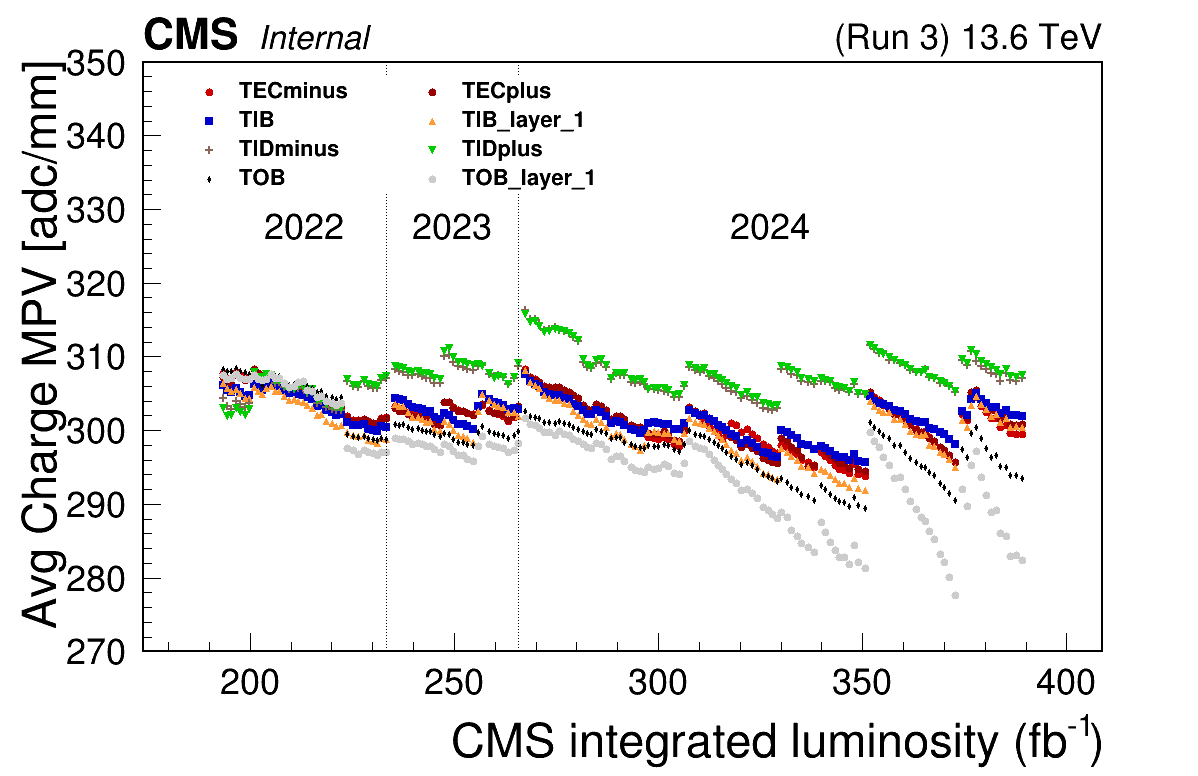
\includegraphics[width=0.8\textwidth]{figures/CalibratedCharge_run3_lumi.png}
   \caption{Time evolution of the calibrated SiStrip cluster charge as a function of the integrated luminosity during LHC Run 3, shown separately for different detector regions. Discontinuities in the trends correspond to periodic re-calibrations. The increasing deviations from the nominal calibration value of 300 ADC/mm highlight the impact of silicon sensor and readout fiber ageing, emphasizing the need for more frequent calibration updates to maintain optimal detector performance.}
   \label{fig:StripClusterCharge}
\end{figure}

\subsubsection{CPE Conditions}

\begin{itemize}
    \item Two key CPE-related conditions are maintained:\newline
    \texttt{SiStripLorentzAngleRcd} and \texttt{SiStripBackPlaneCorrectionRcd}.
    \item Both conditions are provided in two configurations: "deconvolution" and "peak," depending on the readout mode.
    \item Updates to these calibrations require dedicated workflows involving special datasets (e.g., cosmics, low pile-up collisions).
    \item The conditions have seen minimal updates since early Run 2, as miscalibrations are often treated as geometric mispositioning during tracker alignment procedures.
    \item A monitoring workflow exists in the Prompt Calibration Loop (PCL), but direct calibration at HLT is limited.
\end{itemize}

\subsubsection{NGT Demonstrator Candidate Evaluation}

To summarise the main NGT calibration workflow candidates:
\begin{itemize}
    \item \textbf{Bad Components Masking}:
    \begin{itemize}
        \item Already implemented in PCL workflows and requires minimal statistics for updates.
        \item Demonstrated to improve track building in inside-out muon reconstruction.
    \end{itemize}
    \item \textbf{Particle Gains Calibration (a.k.a. G2)}:
    \begin{itemize}
        \item High-statistics requirement makes frequent updates infeasible.
        \item Potential minor impact on track building and cluster charge thresholds.
    \end{itemize}
\end{itemize}

The recommendations in the context of the NGT calibration workflow are:
\begin{itemize}
    \item Prioritise the inclusion of bad components masking in the NGT demonstrator workflow due to its operational simplicity and demonstrated impact.
    \item Consider periodic evaluations for integrating gain calibrations as part of long-term upgrades.
\end{itemize} % Marco
%!TEX root = ../main.tex
\subsection{ECAL Calibrations}\label{sec:ECALlaser}

The energy $E$ deposited in each electromagnetic calorimeter (ECAL) crystal is reconstructed according to 
\[
E = A \cdot G \cdot LC(t) \cdot C(t),
\]
where
$A$ is the digital signal amplitude above the \emph{pedestals},
$G$ is a conversion factor from ADC counts to \GeV,
$LC(t)$ are the \emph{laser corrections} that account for the effect of irradiation of the crystals due to the LHC collisions, and
$C(t)$ is a combinations of calibration constants that account for the different crystal and photodetector responses, \textit{i.e.} the \emph{intercalibrations}.
These aim to equalise the ECAL response both for different crystals at the same $\eta$ coordinate,
and
the absolute scale as a function of $\eta$.
Finally, the measurement of the electronic \emph{pulse shapes} themselves is also paramount to the ECAL calibration, not only for the measurement of the deposit energy but also for the \emph{timing capabilities} of the subdetector.
A more detailed description of
the operation and performance of the CMS ECAL,
including calibration procedures,
is available in Ref.~\cite{CMS:2024ppo}.

%%% I don't know how much I believe these numbers here.
Out of the 326 conditions in the HLT GT,
67 are related to ECAL, %59
of which 52 are relevant to \Runthree data-taking. %36
From these, the following are considered core and critical for data-taking:
\begin{table}[h!]
    \centering
    \begin{adjustbox}{max width=\textwidth}
    \begin{tabular}{p{3.5cm}|p{4.5cm}|p{2.5cm}|p{2cm}|p{4cm}}
        \textbf{Name} & \textbf{Record} & \textbf{Workflow} & \textbf{Frequency of Updates} & \textbf{Description} \\ \hline
    Laser corrections & \texttt{EcalLaserAPDPNRatios} & ECAL automation and manual & Every 40 min or per fill & Crystal transparency and photodetector response. \\
    Pedestals & \texttt{EcalPedestals} & PCL and ECAL automation & Per run or weekly & Pedestals for noise measurements. \\
    Pulse shapes & \texttt{EcalPulseShapes} & ECAL automation and manual & 3 days & Pulse shapes. \\
    Timing & \texttt{EcalTimeCalibConstants} & ECAL automation and manual & Weekly & Time of the pulse maximum.\\
    Intercalibrations & \texttt{EcalIntercalibConstants} & ECAL automation and manual & Weekly or more & Equalise crystal response vs. $\eta$ and $\phi$.
    \end{tabular}
    \end{adjustbox}
    \caption{Fundamental ECAL Calibrations, ordered in terms of frequency of updates.}
    \label{tab:ECALCalibrations_critical}
\end{table}

\subsubsection{Pedestals}

%EcalPedestalsRcd

The ECAL pedestals represent the baseline from which the electronics pulses are measured.
Pedestals are measured for the three possible configurations (gains) of the multi-gain preamplifier integrated in the ECAL readout chip: $\times 1$, $\times 6$ and $\times 12$.
In the offline tag,
the PCL updates the G12 pedestals automatically, while
the G1 and G6 pedestals are updated manually every week.
In the online tag, all three pedestals are updated manually weekly.

\subsubsection{Laser Corrections}

%EcalLaserAPDPNRatiosRcd

The transparency of the ECAL crystals and the photodetector's response to light are degraded as an effect of the irradiation from the LHC collisions.
The degradation as a function of time is monitored crystal by crystal by measuring the response to the light of a laser system.
The light is injected in the system during the LHC abort gap, and a complete scan of the calorimeter takes 40 minutes.
The measurement of the response degradation is then used as a correction factor in the energy reconstruction.
In the offline tag, this correction is available with that same 40-minutes granularity,
while in the online tag it is available only once per LHC fill.
Figure~\ref{fig:ECALTransparency} shows the ECAL relative response to the laser light,
as a function of time,
for the LHC \Runtwo.
We can see that the more forward sections of the subdetector show the largest response decrease as expected, due to the strongest irradiation to which they're subjected.
\begin{figure}[htbp]
   \centering
   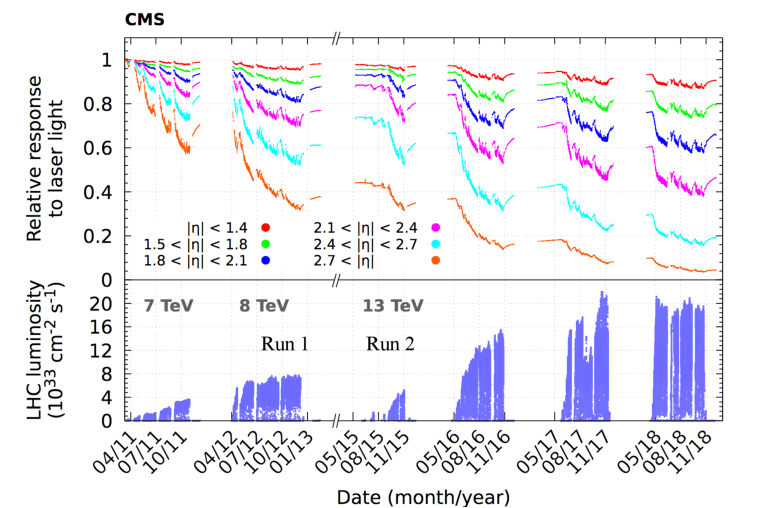
\includegraphics[width=0.7\textwidth]{figures/ECALTransparencyEvolutionRun2.pdf}
   \caption{ECAL relative response to the laser light, as a function of time, for the LHC \Runtwo.
   The LHC instantaneous luminosity is also shown in the lower panel.
   Figure extracted from Ref.~\cite{CMS:2024ppo}.
}
   \label{fig:ECALTransparency}
\end{figure}

\subsubsection{Pulse Shapes}

%EcalPulseShapesRcd

The ECAL pulse shapes also change because of the irradiation affects,
and those changes also directly change the reconstruction of the signal amplitude.
These updates are more critical after a technical stop of the LHC.
The same payloads are used in the offline and online tags.

\subsubsection{Timing Corrections}

%EcalTimeCalibConstantsRcd

The fast signal from the crystal scintillation enables the ECAL subdetector to provide timing measurements in addition to energy.
In test beam conditions, the ECAL barrel achieved a 100\,ps precision for energy deposits above 10--20\GeV.
Effects from clock distribution variance,
instabilities in clock initialisation in different readout units,
and crystal degradation
decrease that precision to 180--350\,ps range.
The ECAL timing drifts
towards negative times during collisions
and
towards positive times during recovery.
For the current standard used for the calibration (ratio timing),
the same payloads are used in the offline and online tags.

\subsubsection{Intercalibrations}

%EcalIntercalibConstantsRcd

The intercalibrations are derived for each crystal and employ a series of methods:
the azimuthal symmetry of the energy deposits in ECAL,
the known mass of particles that decay to electrons and photons
($\text{Z}\to\text{ee}$, $\pi^0\to\gamma\gamma$),
and
the energy--momentum ratio ($E/p$) of electrons from electroweak boson decays.
In general these calibrations require multiple inverse femtobarns of integrated luminosity to derive;
the same payloads are used in the offline and online tags.

\subsubsection{Alignment}

Alignment of the ECAL with respect to the Tracker system is done infrequently,
mainly when there is a cycle of the CMS magnet.
We will not consider alignment conditions for subdetectors other than the Tracker for further discussion in this report.

\subsubsection{NGT Demonstrator Candidate Evaluation}

In view of the above discussion, we consider the \emph{laser corrections} a possible candidate for the implementation in NGT.
The gap between online and offline update frequencies (40 minutes vs. per fill) is large enough that, in principle, expressive improvements can be realised by improving the online calibration.
 % Thiago
\subsection{HCAL Calibrations}

The calibration of the hadron calorimeter (HCAL) is vital in the determination of the energy scale and resolution of hadrons, and consequently jets and missing transverse momentum \cite{CMS-PRF-18-001}.

There are no HCAL calibrations included in the PCL, however, there exist HCAL automation workflows (discussed in Section \ref{sec:CMScalibration}) that update HCAL conditions on a weekly basis (e.g. gains, pedestals). Most conditions are explicitly incorporated into the Look-Up Tables (LUTs) that are loaded on-detector and append the GT via the O2O procedure semi-automatically (discussed in Section \ref{sec:CMScalibration}). The remaining conditions are updated rarely (yearly or less-frequent) and uploaded manually to the conditions database. Many HCAL conditions are also relevant for L1T and the corresponding trigger primitives. Out of the 326 conditions in the HLT GT, 37 are related to HCAL, of which 24 are relevant to Run 3 data-taking. From these, the following 7 are generally considered core and critical for data-taking:

\begin{table}[h!]
    \centering
    \begin{adjustbox}{max width=\textwidth}
    \begin{tabular}{p{3.5cm}|p{4cm}|p{2.5cm}|p{2cm}|p{4.5cm}}
        \textbf{Name} & \textbf{Record} & \textbf{Workflow} & \textbf{Frequency of Updates} & \textbf{Description} \\ \hline
        Gains (RadDam) & \texttt{HcalGains} & O2O & Weekly & Response corrections for radiation damage (RadDam). \\
         Pedestals & \texttt{HcalPedestals} & HCAL automation (O2O) & Weekly & Pedestals for noise measurements.\\
        Pedestal Widths & \texttt{HcalPedestalWidths} & HCAL automation (O2O) & Weekly & Pedestals for noise measurements. \\
        L1T Trigger Objects & \texttt{HcalL1TriggerObjects} & HCAL automation (O2O) & Weekly & L1T trigger objects, including relevant conditions: pedestals, gains and response corrections, channel quality. \\
        Response Corrections & \texttt{HcalRespCorrs} & O2O & per Era ($\approx 20~\fbinv$) & Corrections to detector energy response. \\
        Channel Quality & \texttt{HcalChannelQuality} & O2O & Few times per year & Tracking of dead or non-functional HCAL cells. \\
        Geometry Parameters & \texttt{HcalParameters} & Manual & Yearly & Parameters containing the HCAL geometry. \\
        %Look-Up Table (LUTs) Corrections & \texttt{HcalLUTCorrs} & O2O & Rarely & Corrections related to Look-Up Tables (LUTs). \\
    \end{tabular}
    \end{adjustbox}
    \caption{Fundamental HCAL Calibrations, ordered in terms of frequency of updates.}
    \label{tab:HCALCalibrations_critical}
\end{table}

In the context of an optimal calibrations workflow, the first 6 from Table \ref{tab:HCALCalibrations_critical} are considered fundamental and generally require more frequent updates. These have been analysed in more detail in the following sections. % NOTE: footnote could be moved to Others section.

\subsubsection{Response Corrections}
Response corrections (\texttt{HcalRespCorrs}) \cite{CMS-PRF-18-001} are calibrations that aim to equalise the signal coming from the detector to provide a uniform energy measurement. Some knock-on effects of other miscalibrations such as time misalignment, can also be reflected and absorbed by these corrections. They have a very significant effect on HLT reconstruction and rates, and thus are considered critical. Generally, they are updated roughly every era ($\approx 20 \fbinv$), however, the exact frequency depends on the HCAL subsystem and type of correction. Generally, the required statistics determines the frequency, as the analyses are often statistically-limited. The updates are explicitly incorporated into the LUTs that are loaded on-detector and the corresponding conditions appended to HLT GT via the O2O procedure semi-automatically (discussed in Section \ref{sec:CMScalibration}).
% Technically-speaking, if the calibrations are determined accurately, they would require less-frequent updates (modulo any hardware changes).

% HB and HE
The main calibrations for the hadron barrel (HB) and hadron endcap (HE) calorimeters come in in two forms: azimuthal ($\phi$\texttt{-symmetry}) and isolated track (\texttt{IsoTrack}) corrections, which are multiplicative factors. 

% Azimuthal (Phi-)Symmetry
Asymmetries in the response over $\phi$ arise due to structure, materials, inhomogeneous magnetic field, beamspot shifts, and miscalibrations. The $\phi$\texttt{-symmetry} intercalibrations equalize the detector response in $\phi$ for each $i\eta$ ring and depth section of the HCAL. They take advantage of the uniformity of particle energies across the azimuthal angle $\phi$. An intercalibration is performed between calorimeter channels by comparing it to the average collected energy in the entire $i\eta$ ring. Two methods are used to determine them, depending on the hadron energies:
\begin{itemize}
    \item For high energies ($> 4 \GeV$) an iterative method is used, where scale factors for uncalibrated energies are determined iteratively by equalizing the mean of the energies in an energy interval. An unbiased dataset is used with events triggered by detectors other than HCAL, such as electron, photon and muon triggers. The reconstructed energies are obtained from zero-suppressed events after noise (pedestal) subtraction.
    \item For low energies ($< 4 \GeV$; down to a fraction of a GeV), a method of moments is used, where the first (mean) and second (variance) moments of the energy distribution are compared to that of the entire $i\eta$ ring. This method uses minimum-bias events taken without zero-suppression (NZS). The noise (pedestal) is subtracted from the energy distribution.
\end{itemize}

The uncertainty-weighted average of the scale factors from both methods is used as the final scale factor for the $\phi$-intercalibration.

% Isolated Track (IsoTrack)
An absolute calibration of charged hadrons is performed by comparing the energy measurement with that of the tracker system, taking advantage of the precise calibration of the tracker system. Unlike the tracker momentum measurement, the HCAL energy response is non-linear, especially at lower energies. Therefore, the goal of the calibration is to equalize the relative energy scale for higher momentum charged hadrons that do not interact hadronically with the ECAL. Isolated tracks of hadrons with momenta between $40-60 \GeV$ are used. Data samples are collected using dedicated \texttt{IsoTrack} triggers with special isolation and maximum requirements on the energy deposited in the ECAL, as well as a more standard set of physics triggers with similar selections applied offline. Preferably they are determined in a depth-dependent way (assuming there are no statistical limitations), since in such a form they are more optimal, as indicated in Figure \ref{fig:HCAL-IsoTrack}.

\begin{figure}[h!]	
\centering
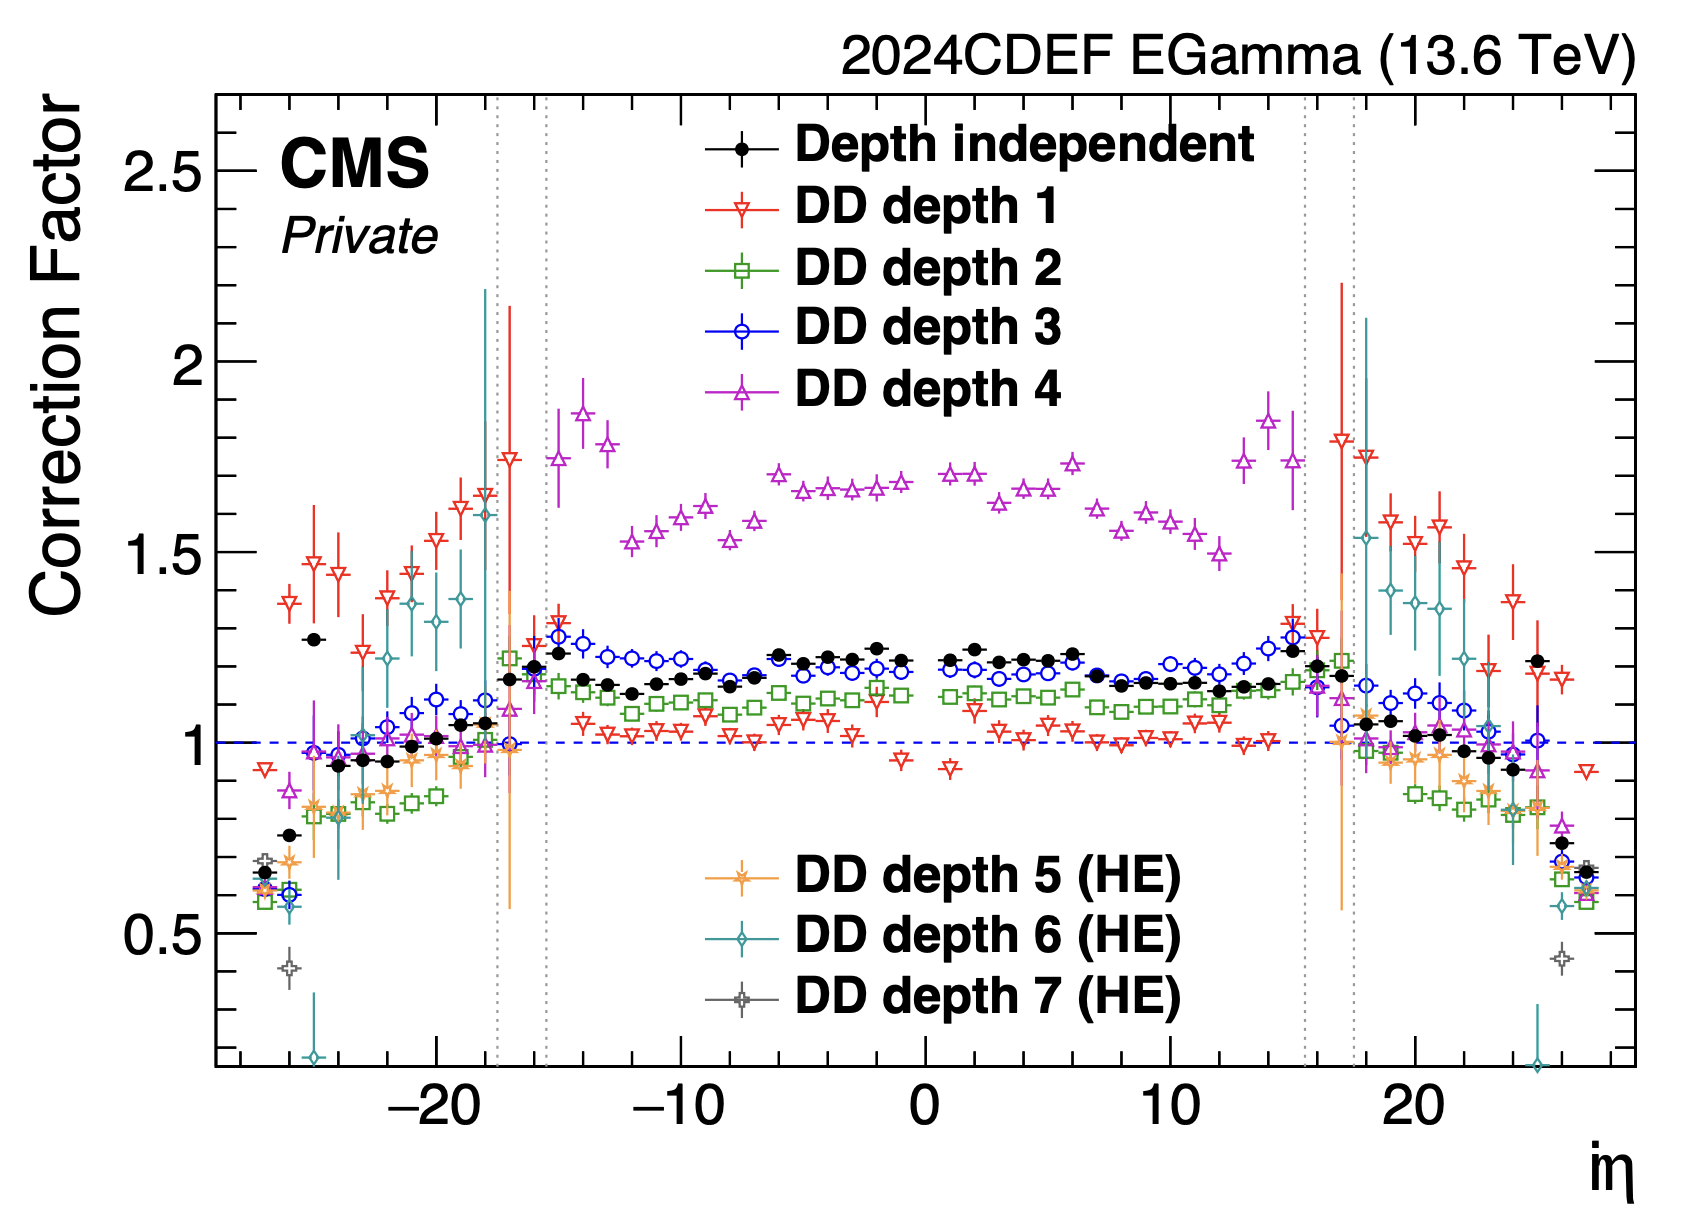
\includegraphics[width=0.7\textwidth]{figures/HCAL_IsoTrack_DepthDependent_2024.png} %\hfill
\caption{HCAL \texttt{IsoTrack} response corrections determined from 2024 data, indicating that depth-dependent ones are more optimal, given their variation across depths.} 
\label{fig:HCAL-IsoTrack}
\end{figure}
% NOTE: this plot is very fresh (Nov. 2024) and CMS-internal/not-approved. From our internal discussions, the consensus is that this should be fine for the purpose of this report. Credits: Jet response: Mikko Voutilainen (analysis+plots), Yildiray Komurcu (HCalRespCorrs payloads), Mikael Myllymäki (re-reco + jet matching); IsoTrack: Sunanda Banerjee (reference code), Jyoti Babbar (HcalIsoTrackAnalyzer tuples), Suman Dasgupta Source: https://indico.cern.ch/event/1475724/contributions/6219567/attachments/2964001/5213972/2024_11_08_HCAL_DepthTo2024ReReco.pdf

% HF
The forward calorimeter (HF) is also calibrated using the $\phi$-symmetry, while the energy scale is extrapolated using $Z \rightarrow ee$ events. The dataset consists of events with one electron candidate in the HF and the other in the ECAL, which has been precisely calibrated. The scale is adjusted so that the dielectron invariant mass corresponding to the Z-peak is consistent between data and simulation.

% HO, ZDC
For HO, the intercalibration makes use of muons from collision data, as well as cosmic ray muons, while the determination of the absolute energy scale makes use of di-jet events. These calibrations are mostly unchanged with respect to initial calibrations.

The Zero-Degree Calorimeter (ZDC) calibrations are also mostly unchanged and are not discussed here further. 

\subsubsection{Gains (RadDam)}\label{sec:HCAL_gains}
The \textit{gains} (or \texttt{RadDam}) calibrations (\texttt{HcalGains}) are responsible for correcting for radiation damage in the HCAL. Generally this leads to a decreased signal due to the darkening of active scintillator material and fibres (similar to the ECAL laser corrections covered in Section \ref{sec:ECALlaser}). Conversely, the recovery process of thermal annealing also effects the signal and needs to be corrected for. Due to the increased radiation in the forward region, primarily HE and HF are corrected. These corrections are especially important in the high $|i\eta|$ regions where there is no tracker coverage and the \texttt{IsoTrack} response corrections are less accurate and cannot cover for these differences. Therefore, they can be considered critical especially for those regions. HB and HO have not been corrected for a long time due to lower radiation damage. The corrections are determined $|i\eta|$- and depth-dependent and $|i\phi|$-independent) yielding a multiplicative factor together with the response corrections for final calibrated response in GeV. Generally, they are updated via the O2O procedure semi-automatically (discussed in Section \ref{sec:CMScalibration}), roughly every era ($\approx 20 \fbinv$), as with the response corrections.

Typically, the measurements of the radiation damage is based on laser data in the orbit/abort gap, when there is no beam in the LHC. The laser system sends light to the photodetectors (SiPMs, PMTs) or directly to the scintillators. The ratio of the amplitudes gives a measure of the signal attenuation. The laser data is then compared to that taken at the start of the yearly data-taking in order to measure the net effects of radiation damage. A new dedicated radiation damage monitoring system was recently developed for the HF quartz fibres. 

The effects of radiation damage are dependent on the delivered luminosity. The dependence is modelled and parametrised to exponential decay~\cite{CMS:2020mce}. An example of the relative laser signal in a single $i\eta$ region and layer is shown in Figure \ref{fig:HCAL-Laser_data}. 

\begin{figure}[h!]	
\centering
\includegraphics[width=0.7\textwidth]{figures/HCAL-Laser_data2024.png} %\hfill
\caption{Laser system data in layer 1, $i\eta = 27$ of the HCAL, indicating the relative signal as a function of the total integrated luminosity L in $\fbinv$, parametrised as exponential decay. The missing data points indicate the extended downtime of the laser system in 2024.}
\label{fig:HCAL-Laser_data}
\end{figure}

In the case of downtime of the laser system (also seen in Figure \ref{fig:HCAL-Laser_data} for 2024), the backup approach are dedicated energy flow extrapolations, which are non-trivial. Therefore, the preference is to use laser data.

\subsubsection{Pedestals}\label{sec:HCAL_pedestals}
The HCAL pedestals (\texttt{HcalPedestals}) and their corresponding widths (\texttt{HcalPedestalWidths}) are essentially measurements of the noise "floor" that are offset to avoid any energy measurement bias. Some sources of noise include dark and leakage currents, or particles interacting with the readout electronics. Generally, it increases with radiation damage. Regular pedestal updates are important to avoid any drifting of HCAL-driven trigger rates and contributions to the fraction of the energy deposited in the HCAL and ECAL, $\frac{H}{E}$, which is an observable used in the identification of electrons and photons, including shower shapes and isolation. The pedestals are also important inputs into other calibrations, such as the response corrections.

Generally, they are updated roughly every week ($\approx 2 \fbinv$), as part of the HCAL automation workflow (discussed in Section \ref{sec:CMScalibration}). Effective pedestals are calculated from collision runs, where good input data from candidate runs is identified and processed within 1 hour after a given LHC fill. The input data is based on measurements in orbit/abort gap when there is no beam in the LHC (similarly to the laser data for the HCAL gains discussed in the previous Section \ref{sec:HCAL_gains}). The conditions are then automatically uploaded to the conditions database via the O2O procedure (discussed in Section \ref{sec:CMScalibration}). Validation in the context of changes to L1T and HLT trigger rates are produced within 2 hours, with an ultimate validation and green-light from AlCa typically after 1-2 days. Given a successful validation, this is followed by deployment at the subsequent LHC interfill period.

\subsubsection{Other Calibrations}
There are several other critical conditions listed in Table \ref{tab:HCALCalibrations_critical}, which have been deemed unsuitable for the NGT calibration workflow. Therefore, they are briefly discussed in the following section with lesser details.

\begin{itemize}
    \item \textbf{Channel Quality} (\texttt{HcalChannelQuality}): is used for the monitoring the status of dead or non-functional HCAL cells. Such cells return zero signal response, so by default it does not have an effect on HLT reconstruction. It is mostly used for \texttt{ReReco} purposes. Therefore, it is not a viable NGT calibration workflow candidate.
    \item \textbf{L1T Trigger Objects} (\texttt{HcalL1TriggerObjects}): includes response corrections, gains, pedestals, and channel quality (dead cells). Designed to store a snapshot of average corrections per channel at the moment where HCAL LUTs \footnote{The conditions relevant to the HCAL LUTs are: \texttt{Pedestals}, \texttt{PedestalWidths}, \texttt{Gains}, \texttt{RespCorrs}, \texttt{ChannelQuality}, \texttt{ElectronicsMap}, \texttt{QIEData}, \texttt{SiPMCharacteristics}, \texttt{LUTMetadata}, \texttt{LUTCorrs}} were generated. It is updated using the HCAL automator framework (discussed in Section \ref{sec:CMScalibration}). Technically, it is primarily used in the HCAL emulator in DQM and online rate validations. Therefore, it is de-facto not critical and not a viable NGT calibration workflow candidate. % This gives CMSSW sufficient information to produce exactly the same LUT that loaded to firmware, without accessing Online Master Data Storage (OMDS) database. % The conditions relevant to L1TriggerObjects are: Pedestals, Gains, RespCorrs, ChannelQuality
    \item \textbf{Zero Suppression} (\texttt{HcalZSThresholds}): contains the zero suppression (ZS) thresholds on signal. ZS is used for suppressing noise by ignoring and preventing the readout of low signals below a given energy threshold. The thresholds are changed directly in the hardware (and consequently LUTs), which ultimately has a significant effect on HLT reconstruction. It is updated using the HCAL automator framework (discussed in Section \ref{sec:CMScalibration}). However, the condition itself is not directly used as input to the reconstruction and only used for bookkeeping purposes. Therefore, it is not a viable NGT calibration workflow candidate.
    \item \textbf{Geometry Parameters} (\texttt{HcalParameters}): contain details on the HCAL geometry. They are updated rather rarely, on a yearly basis, and thus need not frequent online updates as foreseen within an NGT calibration workflow.
\end{itemize}

One important thing to note is that there exist fundamental HCAL conditions or calibrations which can have a significant effect on HLT reconstruction that are implemented in the hardware directly,  while their conditions database records may not be considered critical per se (but rather used for bookkeeping purposes); Examples include the aforementioned zero-suppression thresholds (\texttt{HcalZSThresholds}) or the timing alignment.

\subsubsection{NGT Demonstrator Candidate Evaluation}
In the context of a potential candidates for the optimal NGT calibrations:
\begin{itemize}
    \item The response corrections involve a number of dedicated separate offline analyses for different HCAL subsystems, using various input datasets (incl. \texttt{AlCaRecos}) and specific selections. Thus, their determination is rather convoluted and they are tricky to do without proper offline analysis and corresponding validation. Even though some of the sub-calibrations might be reasonably possible to automate (e.g. $Z \rightarrow ee$ for HF), it would still require a significant amount of work, especially in the context of proper validation. Furthermore, since they are incorporated into the LUTs, they are entangled together with L1T condition updates. Therefore, one can conclude that the response corrections are not a viable candidate for the NGT workflow in their current form, especially for the Run 3 prototype.
    \item The gains (or \texttt{RadDam}) corrections are important for HLT reconstruction and require frequent updates. There are plans to include them in the HCAL automation system (covered in more details the next Section \ref{sec:HCAL_pedestals}) within weekly updates. Therefore, they are a good candidate for the NGT workflow. One caveat is that they are dependent on laser data, which requires a different data stream than the standard bulk collisions data. Furthermore, a vital requirement is a well-functioning laser system.
    \item The pedestals are critical inputs. They are included in the HCAL automation system within weekly updates, which automatically make them a good candidate for the NGT workflow. One caveat is that they are dependent on orbit/abort gap data, which requires a different data stream than the standard bulk collisions data.
\end{itemize}

Therefore, the recommendation is to consider the inclusion of the gains (\texttt{RadDam}) and pedestals in the NGT demonstrator workflow, with the caveat that they require laser data as input. Response corrections are not a viable candidate for the demonstrator in their current format, however, elements could potentially be considered for the future in the context of the \Phasetwo upgrade, under the assumption significant work is invested in its automation and validation. The remaining conditions are not considered viable candidates.

% NOTE: The conditions for Look-Up Tables (LUTs) are: \texttt{Pedestals}, \texttt{Gains}, \texttt{RespCorrs}, \texttt{ChannelQuality}, \texttt{ElectronicsMap}, \texttt{QIEData}, \texttt{SiPMCharacteristics}, \texttt{LUTMetadata}, \texttt{LUTCorrs}

% TODO: more complete list in annex (incl. non-critical calibrations) % Mateusz
\include{chapters/Calibrations_Muons} % Thiago

%\section{Physics Performance} % sadly this needs to be skipped.

%%% Here we discuss the 
%% Physics performance
% Assessment on the impact of non-optimal calibrations on the physics performance of the online reconstruction, by analysing data to quantify the effects of calibration inaccuracies.
